\documentclass[10pt,conference]{IEEEtran}

\ifCLASSINFOpdf
	\usepackage[pdftex]{graphicx}
	%\graphicspath{{./figs/}}
	\DeclareGraphicsExtensions{.pdf,.jpeg,.png}
\else
	\usepackage[dvips]{graphicx}
	%\graphicspath{{./figs/}}
	\DeclareGraphicsExtensions{.eps}
\fi

\usepackage[cmex10]{amsmath}
\usepackage[tight,footnotesize]{subfigure}
\usepackage{xcolor}
\usepackage[lined,ruled]{algorithm2e}

\usepackage[latin1]{inputenc}
\usepackage{tikz}
\usetikzlibrary{shapes}
\usetikzlibrary{arrows}

\usepackage[]{algorithm2e}

\newtheorem{property}{Property}
\newtheorem{proposition}{Proposition}
\newtheorem{theorem}{Theorem}
\newtheorem{conjecture}{Conjecture}
\newtheorem{question}{Question}
\newtheorem{definition}{Definition}
\newtheorem{corollary}{Corollary}

\makeatletter
\pgfdeclareshape{datastore}{
\inheritsavedanchors[from=rectangle]
\inheritanchorborder[from=rectangle]
\inheritanchor[from=rectangle]{center}
\inheritanchor[from=rectangle]{base}
\inheritanchor[from=rectangle]{north}
\inheritanchor[from=rectangle]{north east}
\inheritanchor[from=rectangle]{east}
\inheritanchor[from=rectangle]{south east}
\inheritanchor[from=rectangle]{south}
\inheritanchor[from=rectangle]{south west}
\inheritanchor[from=rectangle]{west}
\inheritanchor[from=rectangle]{north west}
\backgroundpath{
    %  store lower right in xa/ya and upper right in xb/yb
\southwest \pgf@xa=\pgf@x \pgf@ya=\pgf@y
\northeast \pgf@xb=\pgf@x \pgf@yb=\pgf@y
\pgfpathmoveto{\pgfpoint{\pgf@xa}{\pgf@ya}}
\pgfpathlineto{\pgfpoint{\pgf@xb}{\pgf@ya}}
\pgfpathmoveto{\pgfpoint{\pgf@xa}{\pgf@yb}}
\pgfpathlineto{\pgfpoint{\pgf@xb}{\pgf@yb}}
 }
}
\makeatother

\newcommand{\riham}[1]{{\color{red}{#1}}}
\newcommand{\james}[1]{{\color{blue}{#1}}}


\begin{document}

\title{The Rutgers TA Assignment System (RTAS)}

\author{
\IEEEauthorblockN{Wael Ayadi, Nick Romano}
\IEEEauthorblockA{CS526 - Spring 2018 \\
	Rutgers University\\ 
	Piscataway, NJ, USA\\
	Email: wael.ayadi@rutgers.edu, nick.p.romano@gmail.com}
}

\maketitle
\begin{abstract}
\textnormal{
	The Rutgers TA Allocation System (RTAS) is a web application that takes a list of Teaching Assistant (TA) applications as input, processes them using a 3D-Matching algorithm, and allows the user to provide feedback to the algorithm through human-computer interaction in order to extract a collection of approved TA applications that the user is satisfied with. Each TA application is a 3-tuple from the cross-product of three entity sets: the TAs submitting applications, professors, and courses. A generality of this use case is the well known 3D-Matching problem, which is an NP-hard problem where the goal is to find an optimal matching between TAs, professors, and courses. The RTAS will use an approximation algorithm to perform its processing, and it will provide a visual interface that will allow the user to provide feedback to the approximation algorithm in hopes of returning a better output.
}
\end{abstract}
%\onecolumn \maketitle \normalsize \vfill

\IEEEpeerreviewmaketitle
%%%%%%%%%%%%%%%%%%%%%%%%%%%%%%%%%%%%%%%%%%%%%%%%%%%%%%%%%%%%%%%%%%%%%%%%%%%%%%%%%%%%%%%%%%%%%%%%%%%%%%%%%
\section{Project Description}\label{sec:1. Project Description}
The a great number of Rutgers departments allow for graduate students to apply to become Teaching Assistants (TA), where they will be paired up with a professor from that respective department who will act as their mentor, and they will be assigned a course from that respective department that they will be helping to teach. Each TA can only be assigned to one professor and one course, and every professor wants to have a TA that will assist him in his research. Therefore, we would like the maximum number of TA applications approved. However, this is not easy to guarantee, since there can be conflicting TA applications (e.g. two TAs can apply to work under the same professor). As a result, this TA assignment process often tends to be very difficult and tedious. This is because this problem is an example of the 3D-Matching Problem, which one of the well-known NP-hard problems in computational complexity theory. 

This is a 3D-Matching problem, where the three entity sets that are being matched are TAs, professors, and courses. The goal is to find the largest \textbf{matching}, where a matching is a collection of TA applications that do not conflict with each other. Because this problem is NP-hard, the fastest known algorithm for finding a maximum-sized matching has an exponential run-time, which means that it is too slow to be feasible to use in practice. There are approximation algorithms that we can use to derive solutions for the 3D-Matching Problem that are at least a fraction as good as the optimal solution. 

However, the approximation algorithm can output solutions that are quite varied, and normally do not have the means to accommodate for a user's preferences in the matchings. For example, a professor may have had a good experience with a certain TA in the past and prefers that specific TA to work with him over other TAs. However, forcing his preference onto the final matching may result in a final matching that has a smaller size than a final matching without his preference enforced, which can have negative consequences on other professors or courses. 

We propose the Rutgers TA Assignment System (RTAS), which a system that will provide the means to incorporate human-computer interaction into this TA application approval process. The system will provide a visual interface, which will allow for user preferences to be entered. Afterwards, the system will display how the entered user preferences change the quality of the final matching. 

\subsection{Stage1 - The Requirement Gathering Stage. }\label{sec:1 Requirement Gathering Stage. }
%%%%%%%
%\textnormal{
Get a realistic project idea that includes potential real world scenarios,
with a description of the different user types along with their interactions with the system 
as well as the system feedback to them, according to their information needs. 
This stage also requires the specification of the different constraints and restrictions
that need to be enforced depending on the different types of user (system interactions). 
The deliverables for this stage include the following items:
} 

\begin{itemize} 
\item{A general description (in plain English) of your project's deliverables (understandable by computer illiterate users).} 

\item{ A specific description of at least three types of users. }
	
\item{ A description of detailed real world scenarios (at least 2 scenarios) representing those typical interactions between the different user types and the system (including inputs and outputs and data types).}
	

\item{A description of detailed real world scenarios (at least 2 scenarios) representing those typical interactions between the different user types and the system (including inputs and outputs and data types). }

\item{A detailed time line for completion of the major implementaion stages together with the division of labor including testing, documentation, evaluaton, project report, and power point presentation.}

\end{itemize}

Please insert your deliverables for Stage1 as follows:

\begin{itemize} 
\item{The general system description: } 
Please insert the system description here.
\item{The three types of users (grouped by their data access/update rights): }
Please insert the users types in here, as follows:
\item{The user's interaction modes: }
Please insert the user's interaction modes here.
\item{The real world scenarios: }
Please insert the real world scenarios in here, as follows.
	\begin{itemize} 
	\item{Scenario1 description: }
	Please insert Scenario1 description here.
	\item{System Data Input for Scenario1: }
	Please insert System Data Input for Scenario1 here.
	\item{Input Data Types for Scenario1: }
	Please insert Input Data Types for Scenario1 here.
	\item{System Data Output for Scenario1: }
	Please insert System Data Output for Scenario1 here.
	\item{Output Data Types for Scenario1: }
	Please insert Output Data Types for Scenario1 in here.
	\item {Please repeat that pattern for each scenario (at least 2 scenarios per user).}
	\end{itemize}
Please repeat that pattern for each user type.
\item{Project Time line and Divison of Labor.}
Please insert here the time line and the corresponding implementation tasks.
\end{itemize}


\subsection{Stage2 - The Design Stage. }\label{sec: 2:The Design Stage.}
%%%%%%%%%%%%%%%%%%%%%%%%%%%%%%%%%%%%%%%%%%%%%%%%%%%%%%%%%%%%%%%%%%%%%%%%%%%%%%%%%%%%%%%%%%%%%%%%%%%%%%%%%%
\textnormal{This project will use multiple technologies for both the front-end and the back-end. For the back end, we plan to use an SQL database to store the Course, Professor, and TA data. Java servlets will be used for for code execution. For the front-end, we plan on using Angular and Javascript for the layout and D3.js for the visual representation of the 3D matching. We may use jQuery for SQL query manipulation that will serve input to the 3D matching approximation algorithm.}

\begin{figure}
	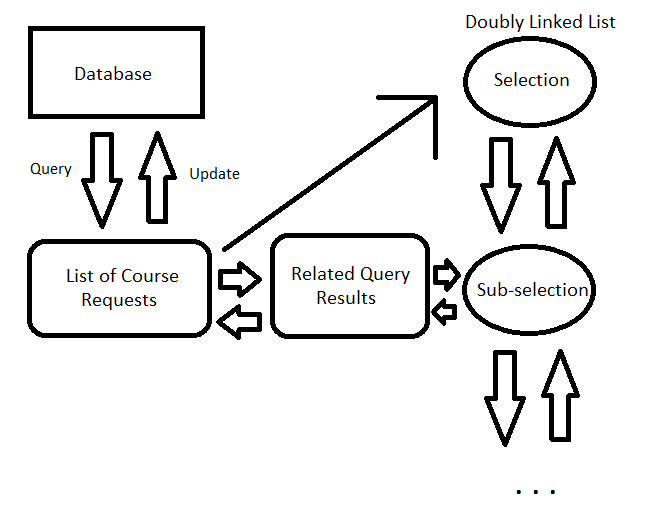
\includegraphics[width=\linewidth]{Data_Structures.png}
	\caption{Internal Data Structures}
	\label{fig:fig1}
\end{figure}

As shown in Figure \ref{fig:fig1}, the back-end operations will be driven by queries to the MySQL database as well as the 3D matching approximation algorithm. The results of the matching algorithm will be fed into the D3.js API that will generate a visual representation of the matching. The user will be able to visualize and manipulate the 3D matching to generate different instances (i.e. solutions) of the matching. When the user selects certain nodes on the interface, such as a specific student or class, those nodes will reference a linked list of triples for which the node belongs allowing the user to quickly visualize local interaction between nodes. The current state of the instance of the 3D matching representation will be stored in a doubly linked list that will allow for progression and regression of the visual interface.  Using a linked list will allow the user to navigate through different instances (solutions) quickly without having to re-run the approximation algorithm.
\\\\

\subsection{Stage3 - The Implementation Stage. }\label{sec: 3 The Implementation Stage.}
%%%%%%%%%%%%%%%%%%%%%%%%%%%%%%%%%%%%%%%%%%%%%%%%%%%%%%%%%%%%%%%%%%%%%%%%%%%%%%%%%%%%%%%%%
The intended programming languages, programming environments, and technologies that will be used for this project have been listed in Stage 2. The remaining deliverables for this section are a work in progress. 


\subsection{Stage4 -	User Interface. }\label{sec: 4. User Interface.}
%%%%%%%%%%%%%%%%%%%%%%%%%%%%%%%%%%%%%%%%%%%%%%%%%%%%%%%%%%%%%%%%%%%%%%%%%%%%%%%%%%%%%%%%%%%%%%%%%%%%%%%%%%
There will be a single primary view for the user interface. The main concept of the user interface is to allow the user to interact with and affect the instance of the TA/Professor/Course matching. This view will contain a representation of the current TA/Professor/Course matching and will allow the user to view the triples in the current instance of the maximal matching. The exact visual representation of the matching will be determined as the project progresses. Several options for interactive visualization are being considered. A graph representation of the matching (where the nodes represent TA's, courses, or professors) may be the most efficient method of providing a visual representation of the entity relationships. The group may consider adapting a hierarchical graph or possibly a radial graph representing all possible sets of TA/Professor/Course triples where the edges between nodes represent possible triples in the maximum matching. The user will be able to interact with the graph by clicking (or hovering) over a node to see the result of the matching. The user will also be able to interact with the current instance of the matching by assigning (or un-assigning) triples. User feedback will trigger the algorithm to recalculate the maximal matching under the user defined assignments and the corresponding visualization will be displayed.  


\end{document}


